% Created 2026-04-23 T5 02:17
% Intended LaTeX compiler: xelatex
\documentclass[11pt,a4paper]{article}
\usepackage[a4paper,margin=2.5cm]{geometry}
\usepackage{fontspec}
\usepackage{polyglossia}
\setmainlanguage{vietnamese}
\setmainfont{DejaVu Serif}
\setsansfont{DejaVu Sans}
\setmonofont{JetBrains Mono}[Scale=0.80]
\newfontfamily\cjkfont{Noto Sans CJK JP}
\usepackage{newunicodechar}
\newunicodechar{五}{{\cjkfont 五}}
\newunicodechar{目}{{\cjkfont 目}}
\newunicodechar{並}{{\cjkfont 並}}
\newunicodechar{べ}{{\cjkfont べ}}
\usepackage{graphicx}
\usepackage{float}
\usepackage{longtable}
\usepackage{tabularx}
\usepackage{wrapfig}
\usepackage{rotating}
\usepackage[normalem]{ulem}
\usepackage{amsmath}
\usepackage{amssymb}
\usepackage{capt-of}
\usepackage{hyperref}
\hypersetup{colorlinks=true,linkcolor=blue,urlcolor=blue,bookmarks=true,bookmarksopen=true,bookmarksopenlevel=1,pdfpagelabels=true}
\usepackage{bookmark}
\usepackage{titlesec}
% Suppress visible section numbers but keep TOC/bookmark entries
\titleformat{\section}{\Large\bfseries}{}{0pt}{}
\titleformat{\subsection}{\large\bfseries}{}{0pt}{}
\titleformat{\subsubsection}{\normalsize\bfseries}{}{0pt}{}
\usepackage{xcolor}
\usepackage{fvextra}
\DefineVerbatimEnvironment{verbatim}{Verbatim}{breaklines=true,breakanywhere=true,fontsize=\footnotesize}
\usepackage[cache=false]{minted}
\usemintedstyle{friendly}
\setminted{fontsize=\footnotesize,breaklines=true,breakanywhere=true,frame=single,framesep=2mm,bgcolor=white,linenos=false,tabsize=2}
\setlength{\parskip}{0.5em}
\setlength{\parindent}{0pt}
\sloppy
\usepackage{graphicx}
\usepackage{longtable}
\usepackage{wrapfig}
\usepackage{rotating}
\usepackage[normalem]{ulem}
\usepackage{capt-of}
\usepackage{hyperref}
\author{larvartar}
\date{\today}
\title{Báo cáo đồ án cuối kỳ — Trò chơi Caro (Gomoku)\\\medskip
\large Môn Nhập môn Lập trình Hướng đối tượng}
\hypersetup{
 pdfauthor={larvartar},
 pdftitle={Báo cáo đồ án cuối kỳ — Trò chơi Caro (Gomoku)},
 pdfkeywords={},
 pdfsubject={},
 pdfcreator={Emacs 30.2 (Org mode 9.7.11)},
 pdflang={Vietnamese}}
\begin{document}

\maketitle
\tableofcontents

\section{TRƯỜNG ĐẠI HỌC KHOA HỌC TỰ NHIÊN — ĐHQG TP.HCM}
\label{sec:org898178e}

\subsection{KHOA CÔNG NGHỆ THÔNG TIN}
\label{sec:orgc9e3566}

\noindent\rule{\textwidth}{0.5pt}
\section{BÁO CÁO ĐỒ ÁN CUỐI KỲ}
\label{sec:orgd75de68}

\subsection{Đề tài: Xây dựng trò chơi \textbf{Caro (Gomoku)} 15×15 với đồ họa 3D và trí tuệ nhân tạo}
\label{sec:orgade2e9d}

\begin{verse}
\textbf{Môn học:} Nhập môn Lập trình Hướng đối tượng\\
\textbf{Lớp:} Công nghệ giáo dục — Khoa Khoa học liên ngành\\
\textbf{Giảng viên hướng dẫn:} TS. Trương Toàn Thịnh\\
\textbf{Học kỳ:} II — Năm học 2025–2026\\
\textbf{Ngày báo cáo:} \uline{\uline{\_}}\\
\end{verse}

\noindent\rule{\textwidth}{0.5pt}
\subsubsection{Nhóm thực hiện — Nhóm 13}
\label{sec:org983d166}

\begin{center}
\begin{tabular}{rll}
MSSV & Họ và tên & Vai trò chính\\
\hline
25310023 & Nguyễn Hữu Thiện Nhân & Nhóm trưởng — Lập trình toàn bộ source code\\
25310057 & Bùi Thị Minh Hằng & Thiết kế slide thuyết trình, biên tập báo cáo\\
25310043 & Phạm Ngọc Trâm & Thiết kế slide, tổng hợp hình ảnh minh họa\\
\end{tabular}
\end{center}

\noindent\rule{\textwidth}{0.5pt}
\subsection{Lời cảm ơn}
\label{sec:orga923083}

Nhóm chúng em xin gửi lời cảm ơn chân thành đến \textbf{TS. Trương Toàn Thịnh} — giảng viên môn \emph{Nhập môn Lập trình Hướng đối tượng} — đã tận tình chỉ dạy những khái niệm nền tảng về lập trình hướng đối tượng, tư duy phân tách bài toán theo lớp và các kỹ thuật xử lý file trong suốt học kỳ vừa qua. Đồ án Caro là cơ hội để nhóm vận dụng tổng hợp những gì đã học, đồng thời mở rộng sang các kỹ thuật nâng cao — máy trạng thái, đa luồng, đồ họa 3D với raylib, thuật toán tìm kiếm cây trò chơi. Nhóm xin cảm ơn các thành viên đã đồng hành, phân công công việc rõ ràng và hỗ trợ nhau trong những ngày cuối trước hạn nộp. Chúng em rất mong nhận được nhận xét và góp ý của Thầy/Cô để hoàn thiện hơn trong các môn học kế tiếp.

\noindent\rule{\textwidth}{0.5pt}
\section{Chương 1 — Tổng quan về đề tài và công cụ}
\label{sec:org27236ef}

\subsection{1.1 Giới thiệu đề tài}
\label{sec:orgade0e8c}

\textbf{Caro} (Gomoku, \emph{五目並べ} trong tiếng Nhật) là trò chơi bàn cờ cổ điển Đông Á: hai người chơi lần lượt đặt quân X và O; ai tạo được năm quân liền nhau theo hàng ngang, hàng dọc hoặc đường chéo trước sẽ thắng. Nếu bàn kín chưa phân thắng bại, ván hòa.

Nhóm chọn biến thể \textbf{Free Gomoku 15×15 không cấm nước} vì: (1) bàn 15×15 đủ lớn để minh họa các kỹ thuật OOP mà không biến đồ án thành bài toán hiệu năng AI; (2) không gian trạng thái \(3^{225}\) cho phép hàm lượng giá heuristic và minimax tạo ra nhiều mức độ thách thức; (3) luật có nhiều biến thể (Renju, Standard Gomoku) nên mở rộng sau này dễ dàng.

Đề tài tích hợp \textbf{nhiều thành phần không đồng nhất} — rules engine, AI (game tree search), đồ họa 3D, file I/O có checksum, giao diện tương tác — là cơ hội chuyển từ tư duy thủ tục sang tư duy hướng đối tượng.
\subsection{1.2 Môi trường và công cụ phát triển}
\label{sec:org60096ba}

\begin{center}
\begin{tabularx}{\textwidth}{lXX}
Thành phần & Lựa chọn của nhóm & Vai trò\\
\hline
Ngôn ngữ & \textbf{C++14} (strict, \texttt{CMAKE\_CXX\_STANDARD\_REQUIRED ON}) & Ngôn ngữ chuẩn của môn học\\
Thư viện đồ họa & \textbf{raylib 5.5} (nạp qua \texttt{FetchContent}) & Render 3D, input, audio, window\\
Build system & \textbf{CMake ≥ 3.16} & Quản lý dependency, cross-platform\\
Unit test & \textbf{Catch2 v3.8.0} & Kiểm thử \texttt{Board} + \texttt{AIPlayer}\\
Tăng tốc build & \textbf{ccache} + \textbf{mold} + \textbf{PCH} & Rebuild nhanh khi chỉnh code\\
IDE nhóm & \textbf{CLion} (Linux) + \textbf{Visual Studio 2022} (Windows, nộp bài) & Đáp ứng môi trường yêu cầu\\
\end{tabularx}
\end{center}

\textbf{Lựa chọn raylib} — API tối giản (\textasciitilde{}100 hàm cốt lõi), hỗ trợ 3D sẵn có (model, shader, camera), phù hợp quy mô đồ án sinh viên. \textbf{FetchContent} — không cần cài công cụ bên ngoài; teacher chỉ cần \texttt{cmake -{}-{}build} là xong. Các tối ưu build (ccache / mold / PCH) giảm rebuild từ \textasciitilde{}25 s xuống \textasciitilde{}3 s — không bắt buộc, chỉ phục vụ dev loop.
\subsection{1.3 Yêu cầu chức năng đã đạt được}
\label{sec:org36a1021}

\begin{center}
\begin{tabularx}{\textwidth}{lXlX}
STT & Chức năng & Mức yêu cầu & Trạng thái\\
\hline
1 & Bàn cờ 15×15, luật 5-in-a-row & Bắt buộc & Hoàn thành\\
2 & Chế độ Người vs Người (PvP) & Bắt buộc & Hoàn thành\\
3 & Chế độ Người vs Máy (PvE) & Bắt buộc & 3 mức: Easy / Normal / Hard\\
4 & Kiểm tra thắng / hòa & Bắt buộc & Quét 4 hướng từ nước cuối\\
5 & Lưu / đọc ván cờ & Bắt buộc & 4 slot, nhị phân + CRC32\\
6 & Giao diện thân thiện & Bắt buộc & Menu, Settings, HUD, hoạt ảnh 3D\\
7 & Undo nước đi & Nâng cao & PvP: undo 1; PvE: undo 2\\
8 & Autosave & Nâng cao & Ghi đè \texttt{autosave.caro} sau mỗi nước\\
9 & Settings bền & Nâng cao & \texttt{settings.cfg}\\
10 & Đồ họa 3D camera quỹ đạo & Tự đề xuất & Phong shader, spherical camera\\
11 & Particle effect & Tự đề xuất & 3 loại: placement / landing / celebration\\
12 & Âm thanh & Tự đề xuất & \texttt{AudioManager} dùng raylib Music + Sound\\
13 & Unit test & Tự đề xuất & Catch2 v3\\
14 & AI async (non-blocking UI) & Tự đề xuất & \texttt{std::thread} + \texttt{std::atomic}\\
15 & Chế độ Story (cốt truyện) & Tự đề xuất & Chiến dịch 4 set, linh-vật, boss cheat (Chương 5)\\
16 & Multiplayer LAN + online & Tự đề xuất & TCP; host-authoritative (LAN) / relay (online) (§2.7)\\
\end{tabularx}
\end{center}

\textbf{Định lượng:} \textasciitilde{}10\,000 LOC source trên 24 module \texttt{.cpp} + 24 header. 2 file test Catch2. Build cold \textasciitilde{}180 s (phần lớn build raylib); rebuild \textasciitilde{}3 s.

\noindent\rule{\textwidth}{0.5pt}
\section{Chương 2 — Thiết kế hệ thống}
\label{sec:org8d487ac}

\subsection{2.1 Kiến trúc tổng thể}
\label{sec:org7335809}

Toàn bộ trò chơi chia thành \textbf{24 module nguồn}, mỗi module một cặp file \texttt{.h} / \texttt{.cpp}. Nguyên tắc: \textbf{một lớp — một trách nhiệm} (SRP); phụ thuộc đi một chiều từ screen → \texttt{Game} → hạ tầng (\texttt{Board}, \texttt{Player}, \texttt{Renderer}, \texttt{FileManager}).

\begin{verbatim}
                  main.cpp
                     |
                     v
                 +-------+
                 | Game  |  (finite state machine + main loop)
                 +-------+
       ___________/ | \______________________________
      /   /   |     |     |     |     |     |       |
     v    v   v     v     v     v     v     v       v
  Board  Player AIPlayer Renderer Audio FileMgr  Screens...
    |      ^      |        |               |     (Menu/
    |      |______|        |               |      Game/
    |    (inherit)         |               |      Settings/
    |                      |               |      SaveLoad)
    |                      v               v
Zobrist table         ParticleSystem    .caro files
(64-bit hash)         Fonts (shared)    settings.cfg
\end{verbatim}

Thiết kế này mang lại: \textbf{Testable} — \texttt{Board=/=Player=/=AIPlayer} không phụ thuộc raylib, tách thành thư viện \texttt{GameLogic} và test bằng Catch2; \textbf{Maintainable} — sửa một module không ảnh hưởng module khác; \textbf{Extensible} — thêm \texttt{NetworkPlayer} hay \texttt{ReplayPlayer} chỉ cần kế thừa \texttt{Player} và override \texttt{getMove}. Hai nhóm tính năng mở rộng gần đây cũng theo đúng nguyên tắc này: \textbf{Multiplayer} (\texttt{NetworkSession}, \texttt{ServerConfig}, \texttt{MultiplayerScreen} — §2.7) và \textbf{Story Mode} (\texttt{StoryMode}, \texttt{StoryContent}, \texttt{StorySigil}, \texttt{ViewBackgrounds} — Chương 5), đều cắm vào máy trạng thái và pipeline \texttt{applyMove} sẵn có mà không sửa lõi \texttt{Board} / \texttt{AIPlayer}.
\subsection{2.2 Máy trạng thái và vòng lặp chính}
\label{sec:org52420de}

Trò chơi được mô hình hóa như FSM. Phiên bản hiện tại có \textbf{11 trạng thái}: 6 trạng thái lõi cộng \texttt{PickDifficulty} (chọn độ khó PvE), \texttt{Multiplayer} (sảnh mạng — §2.7), và 3 trạng thái Story (\texttt{StoryPickSet}, \texttt{StoryIntro}, \texttt{StoryBeat} — Chương 5):

\begin{minted}[breaklines=true,breakanywhere=true,fontsize=\footnotesize,frame=single,framesep=2mm,tabsize=2]{cpp}
enum class GameState {
    Menu, Settings, PickDifficulty, Multiplayer, Playing, GameOver,
    SaveScreen, LoadScreen,
    StoryPickSet, StoryIntro, StoryBeat
};
\end{minted}

\begin{verbatim}
             +----------+
(launch) --> |   Menu   | <-----------------------+
             +----+-----+                         |
                  | New Game / Load Game          |
                  v                               | ESC
             +----+-----+         Ctrl+S          |
+----------> | Playing  |------> [SaveScreen]-----+
|            |          |         Ctrl+L          |
|            |          |------> [LoadScreen]-----+
|  Reset /   +----+-----+         ESC
|  Play Again     | Win / Draw
|                 v
|            +---------+
+------------+GameOver |
             +---------+
\end{verbatim}

Sơ đồ trên minh họa \textbf{vòng lặp lõi}. Ngoài ra, từ \texttt{Menu} còn rẽ sang \texttt{PickDifficulty} (chọn độ khó trước khi vào \texttt{Playing}), \texttt{Multiplayer} (sảnh kết nối mạng — §2.7), và chuỗi Story \texttt{StoryPickSet} → \texttt{StoryIntro} → \texttt{StoryBeat} → \texttt{Playing} (chi tiết ở Chương 5).

Vòng lặp chính \texttt{Game::run()} chia rõ hai phase \textbf{update} (xử lý input, đổi trạng thái) và \textbf{draw} (render theo trạng thái hiện tại), đều phân nhánh theo \texttt{state}. Tách rõ rệt để tránh một cú click làm trạng thái thay đổi giữa lúc đang vẽ. Chạy ở \textbf{60 FPS} qua \texttt{SetTargetFPS(60)}.

\begin{minted}[breaklines=true,breakanywhere=true,fontsize=\footnotesize,frame=single,framesep=2mm,tabsize=2]{cpp}
// Pseudocode — main loop
while (!WindowShouldClose()) {
    switch (state) { /* updateMenu / updatePlaying / ... */ }
    BeginDrawing();
      switch (state) { /* drawMenu / drawPlaying / ... */ }
    EndDrawing();
}
\end{minted}
\subsection{2.3 Mô hình bàn cờ và Zobrist hashing}
\label{sec:org505b7b1}

Lớp \texttt{Board} đóng gói \emph{trạng thái thuần logic} — không phụ thuộc raylib — để tái sử dụng được trong unit test.

\begin{minted}[breaklines=true,breakanywhere=true,fontsize=\footnotesize,frame=single,framesep=2mm,tabsize=2]{cpp}
enum class CellState { Empty = 0, PlayerX = 1, PlayerO = 2 };
struct Move { int row; int col; };

class Board {
    static const int SIZE = 15;
    CellState cells[SIZE][SIZE];   // mảng tĩnh, cache-friendly
    Move      lastMove;            // cho incremental win-check
    uint64_t  zobristHash;         // incremental 64-bit hash
};
\end{minted}

Ba thiết kế quan trọng: (1) \texttt{cells} là mảng tĩnh 2-D — O(1) access, serialize bằng một lệnh \texttt{fwrite}. (2) \texttt{lastMove} lưu trữ — \texttt{checkWinner} chỉ quét từ nước cuối thay vì toàn bàn (xem §3.1). (3) \texttt{zobristHash} cập nhật tăng tiến — XOR với giá trị ngẫu nhiên 64-bit gán cố định cho cặp (vị trí, mark); cho phép tra Transposition Table O(1) (xem §3.5).

\textbf{Zobrist} — trước game, sinh bảng ngẫu nhiên:

\begin{minted}[breaklines=true,breakanywhere=true,fontsize=\footnotesize,frame=single,framesep=2mm,tabsize=2]{cpp}
// Pseudocode — khởi tạo một lần
std::mt19937_64 rng(0x12345678);   // seed cố định → reproducible
uint64_t zobristTable[SIZE][SIZE][2];  // 15×15×2 mark
// ... điền bằng rng()
\end{minted}

Đặt quân \texttt{mark} tại \texttt{(r, c)} → XOR \texttt{zobristTable[r][c][mark]} vào \texttt{zobristHash}. Undo → XOR lần nữa; vì XOR là \textbf{involution}, hash tự động trở về giá trị trước. Seed \texttt{0x12345678} cố định đảm bảo trạng thái giống nhau → hash giống nhau → TT hoạt động đúng và kiểm thử lặp lại được.
\subsection{2.4 Kế thừa và đa hình — \texttt{Player} / \texttt{AIPlayer}}
\label{sec:org6fc0613}

Đây là phần thể hiện trực tiếp ba trụ cột OOP: \textbf{kế thừa, đa hình, đóng gói}.

\begin{minted}[breaklines=true,breakanywhere=true,fontsize=\footnotesize,frame=single,framesep=2mm,tabsize=2]{cpp}
// Pseudocode — bộ khung lớp
class Player {
public:
    virtual ~Player() = default;
    virtual Move getMove(const Board& board);  // virtual!
protected:
    std::string name;
    CellState   mark;
};

class AIPlayer : public Player {
public:
    Move getMove(const Board& board) override;  // override
    // ... TT, pattern table, debug info
};
\end{minted}

Trong \texttt{Game::updatePlaying}, code client gọi đa hình:

\begin{minted}[breaklines=true,breakanywhere=true,fontsize=\footnotesize,frame=single,framesep=2mm,tabsize=2]{cpp}
Player* currentPlayer;  // trỏ đến player1 hoặc player2
Move m = currentPlayer->getMove(board);   // late binding qua vtable
applyMove(m);
\end{minted}

Biểu thức \texttt{currentPlayer->getMove(board)} không biết đối tượng là người thật hay máy. Ở \textbf{runtime}, con trỏ vtable được tra: trỏ tới instance \texttt{Player} → gọi \texttt{Player::getMove} (đọc \texttt{nextMove} do input set sẵn); trỏ tới \texttt{AIPlayer} → gọi \texttt{AIPlayer::getMove} (chạy minimax/greedy).

\texttt{Game} không cần \texttt{if (isHuman) ... else ...} rải rác. Thêm \texttt{NetworkPlayer} (nhận nước từ socket) hay \texttt{ReplayPlayer} (đọc từ log) chỉ cần viết lớp mới kế thừa \texttt{Player}; \textbf{toàn bộ \texttt{Game.cpp} không sửa một dòng} — đúng tinh thần \textbf{Open-Closed} trong SOLID.
\subsection{2.5 Quản lý lưu / đọc file nhị phân}
\label{sec:org4e7a6bc}

Mỗi file save \texttt{.caro} là khối nhị phân gồm header + body, ghi bằng một lệnh \texttt{fwrite(\&data, sizeof(SaveData), 1, fp)}:

\begin{center}
\begin{tabularx}{\textwidth}{lllX}
Offset & Trường & Kiểu & Ý nghĩa\\
\hline
0 & \texttt{magic} & \texttt{uint32\_t} & \texttt{0x4341524F} = ASCII "CARO" — nhận dạng\\
4 & \texttt{version} & \texttt{uint16\_t} & Phiên bản định dạng (hiện tại \texttt{4})\\
8 & \texttt{checksum} & \texttt{uint32\_t} & CRC32 toàn bộ nội dung sau trường này\\
12 & \texttt{timestamp} & \texttt{int64\_t} & Unix timestamp\\
20 & \texttt{playTime} & \texttt{float} & Tổng thời gian chơi (giây)\\
24 & \texttt{moveCount}, \texttt{gameMode}, … & — & Meta: số nước, mode, \texttt{aiDepth}, lượt, stats\\
… & \texttt{story\ldots} & \texttt{int × 6} & \textbf{(v4)} \texttt{storySetId}, \texttt{storyMatchWins/Losses}, \texttt{story\{Voi,Ga,Ngua\}Charges}; \texttt{-1/0} nếu không phải ván Story\\
… & \texttt{cells[15][15]} & \texttt{int[225]} & Trạng thái từng ô\\
… & \texttt{lastMoveRow}, \texttt{lastMoveCol} & \texttt{int × 2} & Phục vụ \texttt{checkWinner}\\
\end{tabularx}
\end{center}

\textbf{Lý do chọn nhị phân nguyên khối} (thay vì JSON/XML): tốc độ (không cần parser), kích thước (\textasciitilde{}1 KB vs \textasciitilde{}3–4 KB JSON), không có parse overhead.

\textbf{Robustness — 3 lớp bảo vệ:}

\begin{enumerate}
\item \textbf{Magic number} \texttt{0x4341524F} — phát hiện file sai định dạng (ví dụ copy nhầm \texttt{.png}).
\item \textbf{Checksum CRC32} theo chuẩn Ethernet IEEE 802.3, polynomial \texttt{0xEDB88320} (\textasciitilde{}12 dòng code) — phát hiện corruption nội dung. Lưu: tính CRC lên mọi byte trừ trường \texttt{checksum}. Đọc: set \texttt{checksum = 0}, tính CRC, so với giá trị đã lưu.
\item \textbf{Atomic write} bằng 3 bước: \texttt{fwrite} vào \texttt{slot1.caro.tmp} → rename \texttt{slot1.caro} thành \texttt{slot1.caro.bak} → rename \texttt{.tmp} thành \texttt{.caro}. Ở mọi thời điểm luôn tồn tại ít nhất một bản hợp lệ — tránh file cụt nửa chừng khi mất điện.
\end{enumerate}

\textbf{Version migration} — định dạng đã qua \texttt{v2} (\texttt{aiDepth ∈ \{2,3,4\}}) → \texttt{v3} (\texttt{aiDepth ∈ \{1,2,3\}}) → \texttt{v4} (bổ sung khối trường Story Mode). Khi load file phiên bản cũ hơn: verify CRC trên byte gốc \textbf{trước}, sau đó remap \texttt{aiDepth} và nâng \texttt{version = 4}; các trường Story để \texttt{0/-1} (mặc định "không phải ván Story").

\textbf{4 slot} — slot 0 = autosave (\texttt{autosave.caro}, ghi đè sau mỗi nước trong \texttt{Game::applyMove}); slot 1–3 = manual save từ \texttt{SaveLoadScreen}.
\subsection{2.6 Đa luồng cho AI — non-blocking UI}
\label{sec:org3ffe0e4}

\textbf{Vấn đề:} AI Hard (minimax d=3) mất 200 ms–2 s/nước. Chạy đồng bộ trong main loop → cửa sổ đơ, OS có thể báo "Not Responding".

\textbf{Giải pháp} — spawn \texttt{std::thread} riêng cho AI, đồng bộ qua \texttt{std::atomic<bool>}:

\begin{minted}[breaklines=true,breakanywhere=true,fontsize=\footnotesize,frame=single,framesep=2mm,tabsize=2]{cpp}
// Pseudocode — async AI
std::thread       aiThread;
std::atomic<bool> aiThinking{false};
Move              aiResult;

void Game::updatePlaying() {
    if (vsAI && currentPlayer == aiPlayer && !aiThinking) {
        aiThinking = true;
        aiThread = std::thread([this] {
            aiResult   = aiPlayer->getMove(board);   // chạy trên bản sao
            aiThinking = false;                       // atomic release
        });
    }
    if (!aiThinking && aiThread.joinable()) {
        aiThread.join();
        applyMove(aiResult);                          // main thread apply
    }
    // AI đang nghĩ → loop vẫn chạy 60 FPS, HUD vẫn hiện "AI đang suy nghĩ…"
}
\end{minted}

\textbf{Ba điểm đồng bộ:} (1) \textbf{Không share \texttt{Board} mutable} — \texttt{getMove} nhận tham chiếu \texttt{const} và tạo bản sao cục bộ. (2) \textbf{Kết quả truyền qua \texttt{std::atomic<bool>}} — khi main thấy \texttt{aiThinking =} false=, mọi ghi vào \texttt{aiResult} trước đó đã visible nhờ memory ordering; không cần mutex. (3) \textbf{Join ngay khi xong} để không leak thread.

Kết quả: AI Hard tìm \textasciitilde{}800 ms, cửa sổ vẽ đủ \textasciitilde{}48 frame trong khoảng đó; camera vẫn xoay được, HUD cập nhật, UX mượt như game thương mại.
\subsection{2.7 Multiplayer - đối kháng qua mạng}
\label{sec:mp-overview}

Ở §2.4 đã nêu lời hứa Open-Closed: \emph{"thêm \texttt{NetworkPlayer} nhận nước từ socket... toàn bộ \texttt{Game.cpp} không sửa một dòng"}. Tính năng Multiplayer chính là hiện thực hóa điểm mở rộng đó - nước đi của đối thủ ở xa được đưa vào đúng pipeline \texttt{applyMove} sẵn có, lõi \texttt{Board} / \texttt{AIPlayer} không đổi.

\textbf{Ba module phối hợp:}

\begin{itemize}
\item \texttt{NetworkSession} - bọc một socket TCP và một \textbf{luồng nền} (\texttt{std::thread}) chuyên \texttt{recv()}. Đây là tầng vận chuyển duy nhất biết về socket.
\item \texttt{MultiplayerScreen} - trạng thái \texttt{GameState::Multiplayer}: sảnh chờ để chọn Host / Join, nhập IP hoặc mã phòng, hiển thị trạng thái kết nối.
\item \texttt{ServerConfig} - cấu hình relay (host, port) đọc từ biến môi trường; cổng mặc định \texttt{34567}. Tách config khỏi code để đổi địa chỉ relay không cần biên dịch lại.
\end{itemize}

\textbf{Hai topology:}

\begin{enumerate}
\item \textbf{LAN P2P (host-authoritative)} - một máy \emph{host}, máy kia \emph{join} bằng địa chỉ IP. Host giữ \texttt{Board} \textbf{thẩm quyền}: nước của client gửi lên, host kiểm hợp lệ rồi \texttt{APPLY} ngược lại cho cả hai. Tránh hai bàn cờ phân kỳ.
\item \textbf{Online relay} - cả hai peer kết nối tới một \emph{relay server} trung gian: một bên \texttt{CREATE} phòng, bên kia \texttt{JOIN} bằng mã phòng; relay chuyển tiếp \texttt{MOVE} qua lại. (Phần mã relay server không nằm trong repo đồ án - chỉ giao thức phía client.)
\end{enumerate}

\begin{verbatim}
  LAN (host-authoritative):
    HOST                                 CLIENT
  +--------+      MOVE  ----------->   +--------+
  |  Game  |   <-- APPLY (host OK) --  |  Game  |
  +---+----+                           +---+----+
      | Board thẩm quyền                   | Board phản chiếu
      v                                    v
  NetworkSession (luồng nền)         NetworkSession (luồng nền)
      |  recv -> hàng đợi NetEvent        |  recv -> hàng đợi NetEvent
      v  main loop rút ở 60 FPS           v  main loop rút ở 60 FPS

  Online (relay):
    Peer A --CREATE-->  +-------+  <--JOIN code-- Peer B
           <--ROOM----  | Relay |  --WAIT/START->
           <--MOVE----  +-------+  ----MOVE----->
\end{verbatim}

\textbf{Bắc cầu network → game} dùng \textbf{đúng kỷ luật} của AI thread (§2.6): luồng nền không bao giờ chạm trực tiếp vào \texttt{Board}; nó đẩy sự kiện vào một hàng đợi \texttt{NetEvent} có khóa, main loop rút hàng đợi mỗi frame nên UI không bao giờ bị chặn.

\begin{minted}[breaklines=true,breakanywhere=true,fontsize=\footnotesize,frame=single,framesep=2mm,tabsize=2]{cpp}
// Pseudocode - bàn giao network -> game (cùng mẫu với AI thread, §2.6)
struct NetEvent { Type type; Move move; std::string text; };

class NetworkSession {
    std::thread          rxThread;   // recv() chặn sống ở đây
    std::mutex           qMutex;
    std::queue<NetEvent> events;     // luồng nền push, main thread rút
public:
    bool poll(NetEvent& out);        // pop không chặn cho main loop
    void sendMove(Move m);           // serialize "MOVE r c\n"
};

void Game::updateMultiplayer() {
    NetEvent ev;
    while (net.poll(ev)) {           // rút ở 60 FPS, không bao giờ chặn UI
        if (ev.type == NetEvent::Move) applyMove(ev.move);  // cùng pipeline
        // START / INFO / QUIT / ERROR -> đổi trạng thái hoặc hiện toast
    }
}
\end{minted}

\textbf{Giao thức dòng-văn-bản} (mỗi lệnh một dòng kết thúc \texttt{\textbackslash n}) - dễ debug bằng \texttt{nc} / \texttt{telnet}, không cần thư viện serialize:

\begin{center}
\begin{tabularx}{\textwidth}{lX}
Lệnh & Ý nghĩa\\
\hline
\texttt{HELLO} & Bắt tay sau khi nối; trao đổi tên + vai trò\\
\texttt{START} & Bắt đầu ván, chốt ai cầm X / O\\
\texttt{MOVE r c} & Gửi nước vừa đánh (tọa độ ô)\\
\texttt{APPLY} & Host xác nhận nước hợp lệ (host-authoritative)\\
\texttt{CREATE} & (relay) Yêu cầu tạo phòng mới\\
\texttt{JOIN code} & (relay) Vào phòng theo mã\\
\texttt{ROOM code} & (relay) Trả mã phòng về cho host\\
\texttt{WAIT} & (relay) Đang chờ đối thủ vào phòng\\
\texttt{INFO} & Thông điệp trạng thái hiển thị cho người chơi\\
\texttt{ERROR} & Lỗi: phòng đầy, mã sai, mất kết nối\\
\texttt{QUIT} & Một bên rời ván\\
\end{tabularx}
\end{center}

\textbf{Đa nền tảng} - \texttt{NetworkSession} bọc khác biệt OS sau một interface: socket POSIX (\texttt{<sys/socket.h>}) trên Linux/macOS, Winsock2 (\texttt{WSAStartup} + link \texttt{ws2\_32}) trên Windows. Phần còn lại của game không thấy sự khác biệt này.

\textbf{Kết luận thiết kế:} đối thủ ở xa chỉ là \emph{một nguồn nước đi khác} đổ vào \texttt{applyMove} - giống hệt người chơi cục bộ hay AI. Đây là minh chứng sống cho lời hứa Open-Closed ở §2.4: thêm cả một hệ thống mạng mà không sửa một dòng nào trong \texttt{Board} hay \texttt{AIPlayer}.

\noindent\rule{\textwidth}{0.5pt}
\section{Chương 3 — Thuật toán trò chơi và trí tuệ nhân tạo}
\label{sec:org33f6013}

Chương này trình bày các thuật toán cốt lõi: phát hiện thắng, thu hẹp không gian tìm kiếm, hàm lượng giá heuristic, và ba tier AI.
\subsection{3.1 Kiểm tra thắng — \texttt{Board::checkWinner}}
\label{sec:org0b1f2b5}

Sau mỗi nước đi phải kiểm \texttt{ai đã thắng chưa?}. Cách ngây thơ (quét toàn bàn × 4 hướng) tốn O(n²) ≈ 4500 phép mỗi nước — lãng phí khi \textbf{chỉ một ô mới thay đổi}.

\textbf{Tối ưu} — quét từ \texttt{lastMove}, 4 hướng = \{(0,1), (1,0), (1,1), (1,−1)\}:

\begin{verbatim}
      \    |    /
       \   |   /
 ---------(r,c)---------      lastMove = (r, c)
       /   |   \
      /    |    \

Với mỗi (dr, dc):
  count = countDirection(r,c,+dr,+dc,mark) + 1 + countDirection(r,c,-dr,-dc,mark)
  nếu count ≥ 5 → thắng
\end{verbatim}

\begin{minted}[breaklines=true,breakanywhere=true,fontsize=\footnotesize,frame=single,framesep=2mm,tabsize=2]{cpp}
// Pseudocode
int Board::countDirection(int r, int c, int dr, int dc, CellState mark) const {
    int count = 0;
    r += dr; c += dc;
    while (inBounds(r, c) && cells[r][c] == mark) {
        count++;
        r += dr; c += dc;
    }
    return count;
}
\end{minted}

Chi phí: 4 × (độ dài chuỗi) ≤ 20 phép/nước — \textbf{cải thiện \textasciitilde{}200 lần}.
\subsection{3.2 Candidate Move Generation — \texttt{getCandidateMoves}}
\label{sec:org092dcfd}

Bàn 225 ô → branching factor \textasciitilde{}200 → minimax d=3 ≈ 8 triệu node → không khả thi. \textbf{Quan sát:} nước hợp lý thường nằm gần các quân đã có.

\textbf{\texttt{getCandidateMoves(radius = 2)}} trả về mọi ô trống trong bán kính Chebyshev ≤ 2 so với ít nhất một quân đã có. Radius 1 (8 ô) quá hẹp — bỏ qua chặn xa; radius 3 (48 ô) quá rộng — tốn branching. Radius 2 là cân bằng: giữa ván có \textasciitilde{}10-15 quân → \textasciitilde{}30-50 ứng viên → d=3 ≈ 64000 node, xử lý được với α-β.

\textbf{Bàn trống} — trả về ô trung tâm \texttt{(7, 7)} làm nước mặc định.
\subsection{3.3 Hàm đánh giá heuristic — Pattern Scoring Table}
\label{sec:org6d48776}

Mỗi cửa sổ 5 ô có 3 trạng thái (empty / self / opp) → \textbf{3⁵ = 243 cấu hình}, mã hóa theo cơ số 3: \texttt{idx = c0 + c1·3 + c2·9 + c3·27 + c4·81}. Bảng \texttt{patternScore[243]} được pre-compute một lần.

\textbf{Bảng 3.1 — Điểm heuristic cho các mẫu tiêu biểu}

\begin{center}
\begin{tabular}{llr}
Mẫu (S = self, . = empty) & Ý nghĩa & Điểm\\
\hline
\texttt{SSSSS} & 5 liên tiếp — thắng & 100 000\\
\texttt{SSSS.} / \texttt{.SSSS} / \texttt{SSS.S} / … & 4 trong cửa sổ → kề chiến thắng & 15 000\\
\texttt{.SSS.} & 3 liên tiếp, hai đầu mở & 1 500\\
\texttt{SSS..} / \texttt{..SSS} & 3 liên tiếp, một đầu đụng rìa & 1 000\\
\texttt{SS.S.} / \texttt{.S.SS} / \texttt{S.SS.} & 3 rải với 1 khoảng trống & 900\\
\texttt{S.S.S} & 3 rải rất thưa & 400\\
\texttt{SS...} / \texttt{.SS..} / … & 2 kề nhau & 100\\
\texttt{S.S..} / \texttt{.S..S} & 2 không kề & 50\\
\texttt{S....} / \texttt{....S} & 1 quân đơn lẻ & 10\\
có quân đối thủ & cửa sổ bị chặn cho self & 0\\
\end{tabular}
\end{center}

\textbf{Hai điểm quan trọng:} (1) cửa sổ có quân đối thủ → điểm self = 0 vì cửa sổ đã bị \emph{phá}; đây chính là cơ chế tự nhiên khiến chặn có giá trị. (2) \texttt{\_SSS\_} (1500) đáng gấp 1.5× \texttt{SSS\_\_} (1000) vì mẫu 3 mở hai đầu sẽ tạo \emph{song ba}, trong khi 3 bị đè chỉ tạo 4 một đầu.

\textbf{Công thức điểm toàn bàn:}

$$
\text{score} = \sum_{\text{windows}} \Big( \text{score}_{\text{self}}(w) - \alpha \cdot \text{score}_{\text{opp}}(w) \Big),\quad \alpha = 1.5
$$

\textbf{Tại sao nhân 1.5× lên đe dọa đối thủ?} — trong luật Caro đến \emph{lượt đối thủ trước}; nếu không chặn, họ thắng nước kế. Hệ số 1.5× khiến AI ưu tiên phòng thủ khi điểm hai bên cân bằng, phản ánh đúng asymmetric turn order.

\textbf{Incremental / Local evaluation} — \texttt{evaluate} toàn bàn tốn \textasciitilde{}660 cửa sổ. Thay bằng \texttt{computeLocalScore(row, col)} chỉ xét cửa sổ đi qua \texttt{(row, col)} (≤ 20 cửa sổ) — giảm \textasciitilde{}33 lần. Cập nhật tăng tiến: \texttt{boardScoreNew = boardScoreOld − localBefore + localAfter}. Leaf node dùng trực tiếp \texttt{boardScore} thay vì gọi \texttt{evaluate} đầy đủ.
\subsection{3.4 AI Easy — Greedy one-ply với Delta Evaluation}
\label{sec:org51bc04c}

AI Easy (\texttt{searchDepth = 1}) không tìm kiếm cây — duyệt ứng viên, chọn cái có \textbf{delta} lớn nhất:

\begin{verbatim}
for each m in getCandidateMoves():
    before = computeLocalScore(m.row, m.col)
    board.place(m, aiMark)
    after  = computeLocalScore(m.row, m.col)
    board.undo(m)
    delta  = after − before
    if delta > bestDelta: bestMove = m
return bestMove
\end{verbatim}

\textbf{Vì sao dùng delta?} — nước chặn open-three của địch có \texttt{localAfter} nhỏ (chỉ một quân đơn lẻ) nhưng \texttt{localBefore} rất âm (mẫu địch × 1.5); nếu so điểm tuyệt đối, AI sẽ bỏ qua nước này. Delta khôi phục đúng ưu tiên phòng thủ nhờ cơ chế 1.5× đã bao hàm trong \texttt{localBefore}.

\textbf{Bảng 3.2 — Khả năng nhìn thấy của Easy}

\begin{center}
\begin{tabularx}{\textwidth}{XlX}
Loại tình huống & Easy? & Giải thích\\
\hline
Đặt để thắng (tự mở 5) & Có & ưu tiên tuyệt đối\\
Chặn địch chuẩn bị thắng (4 → 5) & Có & delta lớn do \texttt{localBefore} cực âm\\
Chặn open-three & Có & delta dương rõ\\
Fork 2 bước của đối thủ (ngoài 1-ply horizon) & Không & \emph{horizon effect} — đặc tính thiết kế\\
Threat chain 3+ nước & Không & không có tree search\\
\end{tabularx}
\end{center}
\subsection{3.5 AI Normal / Hard — Minimax α-β + Transposition Table}
\label{sec:org6852cd0}

\textbf{Normal} = depth 2, \textbf{Hard} = depth 3. AI là MAX (muốn điểm cao), đối thủ là MIN.

\begin{verbatim}
                        [ MAX ]
                       /   |   \
                     m1    m2    m3         <-- AI chọn
                    /       |      \
                [MIN]    [MIN]    [MIN]
               /  |  \   /  |  \  /  |  \
              (leaf: boardScore)

MAX tối đa MIN con. MIN tối thiểu MAX con.
\end{verbatim}

\textbf{Alpha-Beta pruning} — duy trì α (cận dưới cho MAX) và β (cận trên cho MIN). Tại node MAX: kết quả ≥ β → cắt (MIN tầng trên sẽ không chọn nhánh này). Tại node MIN: kết quả ≤ α → cắt. Với move ordering tốt, độ phức tạp giảm từ O(b\^{}d) xuống O(b\^{}(d/2)).

\textbf{Move ordering} — sort ứng viên giảm dần theo \texttt{scoreMove} (heuristic rẻ: ưu tiên win-detection, sau đó \texttt{computeLocalScore}). AI luôn thử nước \emph{tạo threat hoặc chặn threat} trước → α-β cắt sớm.

\textbf{Incremental scoring} — minimax nhận tham số \texttt{boardScore}; khi đặt quân: \texttt{newScore = boardScore − localBefore + localAfter}. Leaf (depth = 0) chỉ \texttt{return boardScore}. Toàn cây chỉ cần \textbf{một lần \texttt{evaluate} ở gốc}.

\textbf{Transposition Table} — cùng một thế cờ có thể đạt qua nhiều dãy nước (\texttt{S₀ → m1 → m2 = S₀ → m2 → m1}). Cache kết quả bằng TT:

\begin{itemize}
\item \textbf{Khóa:} \texttt{board.getHash()} — Zobrist 64-bit.
\item \textbf{Giá trị:} \texttt{TTEntry \{ int depth; int score; TTFlag flag; Move bestMove; \}}, với \texttt{TTFlag ∈ \{Exact, LowerBound, UpperBound\}}.
\end{itemize}

\textbf{Probe} ở đầu \texttt{minimax}: hit + \texttt{entry.depth ≥ depth} → theo \texttt{flag}: \texttt{Exact} trả \texttt{entry.score} ngay; \texttt{LowerBound} → \texttt{α = max(α, entry.score)}; \texttt{UpperBound} → \texttt{β = min(β, entry.score)}; nếu \texttt{α ≥ β} → cắt. Nếu không cắt được, vẫn dùng \texttt{entry.bestMove} để \textbf{hoist} lên đầu danh sách ứng viên.

\textbf{Store} sau khi duyệt xong: \texttt{flag = Exact}; nếu \texttt{bestEval ≤ origAlpha} → \texttt{UpperBound} (failed low); nếu \texttt{bestEval ≥ beta} → \texttt{LowerBound} (failed high). Lưu \texttt{TT[hash] = \{depth, bestEval, flag, bestMoveHere\}}.

TT được \textbf{clear mỗi turn} (\texttt{transTable.clear()}) — bàn đã thay đổi, phần entries cũ thuộc trạng thái quá khứ; tiết kiệm RAM; dễ debug qua \texttt{ttProbes=/=ttHits=/=ttCutoffs}.

\textbf{Bảng 3.3 — So sánh tier}

\begin{center}
\begin{tabularx}{\textwidth}{Xlll}
Tiêu chí & Easy (d=1) & Normal (d=2) & Hard (d=3)\\
\hline
Thuật toán & Greedy + delta & Minimax α-β + TT & Minimax α-β + TT\\
Nodes/nước (ước lượng) & \textasciitilde{}40 & \textasciitilde{}1 000–3 000 & \textasciitilde{}15 000–60 000\\
Thời gian/nước (giữa ván, laptop) & <5 ms & \textasciitilde{}30–80 ms & \textasciitilde{}200–1500 ms\\
Phát hiện fork 2 bước & Không & Có (một phần) & Có\\
\end{tabularx}
\end{center}

\textbf{Các tier thường dừng ở depth 3} — ở một số thế cờ giữa ván, d=4 có thể mất tới \textasciitilde{}120 s/nước nếu move ordering kém. Vì vậy Easy/Normal/Hard giới hạn ở d≤3 để giữ trải nghiệm tương tác. \textbf{Ngoại lệ:} màn FinalBoss trong Story Mode (§5.4) dùng \textbf{depth 4} để tạo độ khó cao trào — nhờ AI chạy trên luồng riêng (§2.6), thời gian suy nghĩ lâu hơn vẫn không làm treo cửa sổ; độ khó được cân bằng thêm bằng thể thức best-of-3 và cơ chế "thiên vị boss". Các cải thiện sâu hơn (iterative deepening, TT persistence, threat-space search) vượt phạm vi môn học.
\subsection{3.6 Cơ chế Undo}
\label{sec:org04f2ed6}

Stack lịch sử + tính chất \emph{involution} của XOR trong Zobrist:

\begin{minted}[breaklines=true,breakanywhere=true,fontsize=\footnotesize,frame=single,framesep=2mm,tabsize=2]{cpp}
// Pseudocode
struct MoveRecord { Move move; CellState mark; Move prevLastMove; };
std::vector<MoveRecord> moveHistory;   // LIFO
\end{minted}

Undo PvP: pop 1 record. Undo PvE (lượt người): pop 2 (AI + human) — nếu chỉ pop 1 thì AI lại đánh ngay, cảm giác như không undo. Zobrist tự phục hồi nhờ XOR involution — không cần lưu hash vào record.
\subsection{3.7 Debug panel (F3)}
\label{sec:org8a68edd}

Nhấn \textbf{F3} để overlay thống kê AI: mode, depth completed, candidates evaluated, search time, nodes searched, \texttt{ttProbes} / \texttt{ttHits} / \texttt{ttCutoffs} / \texttt{ttHoists} / \texttt{ttFinalSize}, top-5 nước với điểm pre-score và search-score. Panel giúp theo dõi: move ordering có hiệu quả (ttHits cao), TT có đáng giá (\texttt{ttCutoffs / ttProbes > 5\%}), có dư thời gian để tăng depth không.

\noindent\rule{\textwidth}{0.5pt}
\section{Chương 4 — Đồ họa và giao diện}
\label{sec:org70a73fc}

\subsection{4.1 raylib — pipeline đồ họa 3D}
\label{sec:org68618f7}

raylib cung cấp pipeline tối giản: \textbf{window} → \textbf{camera3D} → \textbf{model + texture + shader} → \textbf{framebuffer}. Code 3D đặt giữa \texttt{BeginMode3D(camera) / EndMode3D()}, sau đó overlay 2D UI.

\textbf{Model loading} — bàn và quân load từ \texttt{.glb} (glTF 2.0 binary). Mặc định raylib đặt material rỗng ở index 0 và material thực ở index 1; nhóm set \texttt{model.meshMaterial[0] = 1;} để mesh dùng đúng texture.

\textbf{Phong shader tùy chỉnh} — GLSL nhúng trong code C++: \textbf{gloss shader} cho quân (specular cao → cảm giác đá/sứ), \textbf{matte shader} cho bàn (chỉ diffuse + ambient → cảm giác gỗ). Cả hai dựa trên công thức Phong \(I = k_a I_a + k_d (N \cdot L) I_d + k_s (R \cdot V)^n I_s\); điều chỉnh \texttt{n} và \texttt{k\_s} tạo tương phản thị giác giữa quân và bàn.
\subsection{4.2 Màn hình Menu — \texttt{MenuScreen}}
\label{sec:org7f4025e}

6 lựa chọn: New Game / \textbf{Story Mode} / Load Game / \textbf{Multiplayer} / Settings / Exit. Mỗi item có hitbox rectangle; mouse (\texttt{CheckCollisionPointRec}) và keyboard (\texttt{KEY\_UP=/=KEY\_DOWN=/=KEY\_ENTER}) đồng bộ qua biến chung \texttt{selectedIndex}. Font \texttt{Fonts::title} cho tiêu đề, \texttt{Fonts::bold} cho item — phân cấp thị giác.
\subsection{4.3 Màn chơi — camera quỹ đạo + raycast picking + HUD}
\label{sec:orgbe96feb}

\textbf{Orbital camera} — đặc tả bởi ba tham số: \texttt{angle} (quanh trục Y), \texttt{pitch} (góc ngẩng), \texttt{distance}. Vị trí camera tính bằng tọa độ cầu:

\begin{verbatim}
position.x = target.x + distance · cos(pitch) · sin(angle)
position.y = target.y + distance · sin(pitch)
position.z = target.z + distance · cos(pitch) · cos(angle)
\end{verbatim}

\texttt{target = (0,0,0)} (tâm bàn); \texttt{pitch} clamp trong \texttt{[5°, 85°]} để camera không chui dưới bàn. Input: chuột phải kéo (\texttt{angle=/=pitch}), cuộn (\texttt{distance}), \texttt{Q=/=E} xoay, \texttt{Home} reset, 4 nút ở góc trái dưới.

\textbf{Raycast picking} — click chuột → \texttt{GetScreenToWorldRay(mouse, camera)} tạo tia → \texttt{GetRayCollisionQuad} với 4 đỉnh bàn ở \texttt{y = 0} → \texttt{collision.point.(x, z)} → chia cho \texttt{CELL\_SIZE} ra \texttt{(row, col)}. Bounds check rồi set highlight; nếu ô trống thì \texttt{applyMove}.

\textbf{HUD} — overlay 2D: tên + mark 2 người chơi (highlight lượt), số nước, thời gian chơi, trạng thái "AI đang suy nghĩ…", nhắc phím tắt. Text vẽ bằng font TTF 48pt, scale xuống khi vẽ để sắc nét ở nhiều kích cỡ.
\subsection{4.4 Particle System — \texttt{ParticleSystem}}
\label{sec:org54d6917}

Cài đặt tùy chỉnh, mỗi hạt có vị trí / vận tốc / màu / lifetime / rotation / \texttt{shimmerPhase} / \texttt{Shape ∈ \{Sparkle, Cube, DustRing, Confetti\}}.

Update mỗi frame: \texttt{velocity.y -} gravity · dt=, \texttt{position +} velocity · dt=, \texttt{age +} dt=, \texttt{rotation +} rotSpeed · dt=; remove khi \texttt{age > lifetime}. Draw: alpha lerp theo \texttt{1 − age/lifetime}; \texttt{Sparkle} có biến thiên alpha bằng \texttt{sin(time + shimmerPhase)} tạo lấp lánh.

\textbf{Ba loại emit:}

\begin{itemize}
\item \texttt{emitPlacement(x, y, z, color, count=12)} — 12 hạt sparkle + 4 glowing cube khi đặt quân, bay lên tỏa ra.
\item \texttt{emitLanding(x, z, color)} — 8 hạt dust ring khi quân chạm bàn.
\item \texttt{emitWinCelebration(positions)} — tại mỗi ô thắng phát \textasciitilde{}20 hạt confetti 8 màu rơi với trọng lực.
\end{itemize}
\subsection{4.5 Hiệu ứng thắng}
\label{sec:orgc58ae20}

Khi \texttt{checkWinner} trả về mark khác Empty, \texttt{Game} chuyển sang \texttt{GameOver} và kích hoạt: (1) \texttt{drawWinLine} — đường sáng dần trên 5 quân thắng, alpha 0 → 1 trong \textasciitilde{}0.5 s; (2) \texttt{drawVignette} — overlay tối 4 góc, tập trung chú ý; (3) \texttt{emitWinCelebration}; (4) \texttt{AudioManager::playWinSound}. Kết thúc bằng overlay text "PLAYER X WINS!" + nút "Play Again / Menu".
\subsection{4.6 Âm thanh — \texttt{AudioManager}}
\label{sec:org1e96c4b}

raylib chia audio thành \texttt{Music} (streaming, nhạc nền) và \texttt{Sound} (preload, SFX ngắn). Nhóm dùng: \texttt{music.ogg} (\texttt{UpdateMusicStream} mỗi frame, loop); 3 SFX \texttt{click.wav} / \texttt{place.wav} / \texttt{win.wav}. Phím \texttt{M} toggle mute. Volume music = 0.5, SFX = 1.0 — nhạc không át SFX.
\subsection{4.7 Texture per-piece nạp bất đồng bộ}
\label{sec:org3184ddc}

Mỗi ô có vân gỗ riêng → 225 × 2 = 450 texture PNG. Load đồng bộ → block \textasciitilde{}vài giây, cửa sổ trắng khi khởi động.

\textbf{Giải pháp — async pipeline:} background thread đọc + decode PNG → push raw pixels vào \texttt{pendingUploads} queue (có \texttt{std::mutex}); main thread mỗi frame pop 1–2 và upload GPU bằng \texttt{LoadTextureFromImage}. Kết quả: cửa sổ mở ngay, texture dần đổi từ generic sang vân riêng trong \textasciitilde{}3–5 s đầu, \textbf{không rớt FPS}. Cùng nguyên lý "công việc nặng không làm treo UI" đã dùng cho AI thread (§2.6), áp dụng sang I/O.

\noindent\rule{\textwidth}{0.5pt}
\section{Chương 5 - Chế độ Story (cốt truyện)}
\label{sec:story-mode}

Ngoài cờ tự do, đồ án bổ sung một \textbf{chiến dịch cốt truyện} mang tên \emph{"Cô Sử Tiên"} - biến ván Gomoku đơn lẻ thành hành trình bốn chặng có dẫn truyện, phần thưởng và một trận đấu trùm. Điểm thiết kế cốt lõi: \textbf{toàn bộ chế độ dựng trên hạ tầng sẵn có} - cùng \texttt{Board}, cùng \texttt{AIPlayer}, cùng pipeline \texttt{applyMove} - chỉ thêm một tầng trạng thái mỏng cộng dữ liệu kịch bản. Đây là ví dụ thứ hai (sau Multiplayer §2.7) cho thấy kiến trúc OOP cho phép mở rộng lớn mà không sửa lõi.

\subsection{5.1 Cấu trúc chiến dịch}
\label{sec:story-structure}

Chiến dịch gồm \textbf{4 set}, độ khó tăng dần, mỗi set là một loạt \textbf{best-of-3} (thắng trước 2 ván). Độ khó từng set ánh xạ \textbf{trực tiếp} sang tham số \texttt{aiDepth} của \texttt{AIPlayer} đã có ở Chương 3 - không viết thêm dòng AI nào:

\begin{center}
\begin{tabularx}{\textwidth}{llcX}
Set & Độ khó & \texttt{aiDepth} & Vai trò\\
\hline
1 & Dễ & 1 & Greedy + delta - làm quen\\
2 & Vừa & 2 & Minimax α-β + TT\\
3 & Khó & 3 & Minimax α-β + TT (sâu hơn)\\
4 & FinalBoss & 4 & Trùm cuối - độ khó cao trào (§5.4)\\
\end{tabularx}
\end{center}

\begin{minted}[breaklines=true,breakanywhere=true,fontsize=\footnotesize,frame=single,framesep=2mm,tabsize=2]{cpp}
// Pseudocode - mỗi set chỉ là một cấu hình; AIPlayer dùng lại y nguyên
struct StorySet {
    int   aiDepth;      // 1..4  -> đẩy thẳng vào AIPlayer (Chương 3)
    int   winsNeeded;   // 2     -> best-of-3
    Sigil unlock;       // linh-vật mở khóa ở set này (§5.3)
};
static const StorySet SETS[4] = {
    { 1, 2, Sigil::None }, { 2, 2, Sigil::Voi },
    { 3, 2, Sigil::Ga   }, { 4, 2, Sigil::Ngua },
};
\end{minted}

\subsection{5.2 Máy trạng thái Story}
\label{sec:story-fsm}

Story cắm thêm ba trạng thái vào FSM ở §2.2 - \texttt{StoryPickSet} (màn chọn set), \texttt{StoryIntro} (dẫn truyện đầu set), \texttt{StoryBeat} (nhịp kể giữa các ván / khi thắng / khi thua) - rồi tái dùng chính \texttt{Playing} để đánh cờ:

\begin{verbatim}
 Menu --[Story Mode]--> StoryPickSet --chọn set--> StoryIntro
                                                       |
                                          (đọc dẫn truyện)
                                                       v
                            +----------------------> Playing
                            |                          |
              ván kế tiếp   |                  win / lose ván
              (best-of-3)   |                          v
                            +-------------------- StoryBeat
                                                       |
                                  set chưa ngã ngũ ----+
                                                       |
                              set thắng -> set kế / set thua -> kể kết
\end{verbatim}

Mỗi set theo dõi \texttt{matchWins} / \texttt{matchLosses}; đạt 2 thắng → sang set kế (mở khóa linh-vật mới); thua loạt → nhịp kể thất bại rồi cho chơi lại. Toàn bộ là logic đếm mỏng quanh vòng lặp \texttt{Playing} đã có.

\subsection{5.3 Linh-vật - tái dùng cơ chế sẵn có}
\label{sec:story-sigil}

Phần thưởng tiến trình là ba \textbf{linh-vật} (spirit-animal power), mở khóa dần theo set. Điểm hay về kỹ thuật: mỗi linh-vật \textbf{ánh xạ vào một cơ chế đã tồn tại}, không phải tính năng mới từ đầu:

\begin{center}
\begin{tabularx}{\textwidth}{llcX}
Linh-vật & Mở khóa & Lượt dùng & Cơ chế tái dùng\\
\hline
Voi 9 ngà & Từ Set 2 & 1 & Undo: pop khỏi \texttt{moveHistory} (§3.6)\\
Gà 9 cựa & Từ Set 3 & 3 & Ép AI đánh \textbf{ngẫu nhiên} một nước\\
Ngựa 9 hồng mao & FinalBoss & 1 (tự động) & Tự hồi sinh một lần khi sắp thua trận trùm\\
\end{tabularx}
\end{center}

Số lượt (charges) \textbf{reset đầu mỗi set}, lưu trong save v4 (\texttt{story\{Voi,Ga,Ngua\}Charges} - §2.5). HUD hiển thị ba linh-vật dưới dạng \textbf{ấn tam-thái} (\texttt{StorySigil}): biểu tượng sáng khi còn lượt, mờ khi hết, đổi trạng thái Rest/Focused/Pressed như các nút UI khác.

\subsection{5.4 Màn FinalBoss - độ khó cao trào}
\label{sec:story-boss}

Set 4 dùng \texttt{aiDepth = 4} - sâu hơn mọi tier thường (§3.5). Nhờ AI chạy trên luồng riêng (§2.6), thời gian suy nghĩ lâu hơn vẫn không làm treo cửa sổ; người chơi thấy HUD "AI đang suy nghĩ…" trong khi camera vẫn xoay.

Để tạo cảm giác đối đầu một \emph{yêu trùm}, boss có thêm \textbf{cơ chế thiên vị}: cứ sau mỗi 4 nước của người chơi, boss "ăn" tối đa 4 quân gần nhất của người chơi - hiện thực bằng đúng các thao tác sẵn có của \texttt{Board} (\texttt{removeMove}) và stack \texttt{moveHistory}, không thêm cấu trúc dữ liệu mới:

\begin{minted}[breaklines=true,breakanywhere=true,fontsize=\footnotesize,frame=single,framesep=2mm,tabsize=2]{cpp}
// Pseudocode - sau mỗi 4 nước người chơi, trùm "ăn" tối đa 4 quân gần nhất
void Game::onPlayerMovedInBoss() {
    if (++bossPlayerMoveCounter >= 4) {
        bossPlayerMoveCounter = 0;
        // gỡ tối đa 4 quân người chơi gần nhất khỏi moveHistory + Board
        removeRecentPlayerStones(/*count=*/4);
    }
}
\end{minted}

Độ khó cao trào này được \textbf{cân bằng} bằng hai cơ chế phía người chơi: thể thức best-of-3 (sai một ván vẫn còn cơ hội) và linh-vật Ngựa 9 hồng mao tự hồi sinh một lần (§5.3) - đảm bảo trận trùm khó nhưng không bất khả thắng.

\subsection{5.5 Module và tích hợp lưu game}
\label{sec:story-modules}

Story Mode được tách thành các module riêng theo đúng nguyên tắc SRP ở §2.1:

\begin{center}
\begin{tabularx}{\textwidth}{lX}
Module & Trách nhiệm\\
\hline
\texttt{StoryMode} & Logic chiến dịch: set hiện tại, đếm best-of-3, charges, chuyển trạng thái\\
\texttt{StoryContent} & Dữ liệu kịch bản: lời dẫn intro / thắng / thua từng set, tên linh-vật\\
\texttt{StorySigil} & HUD ấn tam-thái: vẽ ba linh-vật + số lượt còn lại\\
\texttt{ViewBackgrounds} & Nền nghệ thuật theo từng màn / set\\
\end{tabularx}
\end{center}

Tiến trình Story được \textbf{lưu cùng hệ thống save chung}: save v4 thêm khối trường \texttt{storySetId}, \texttt{storyMatchWins/Losses}, \texttt{story\{Voi,Ga,Ngua\}Charges} (§2.5). Một ván Story do đó có thể lưu / đọc lại như mọi ván khác - không có code save riêng cho Story.

\noindent\rule{\textwidth}{0.5pt}
\section{Chương 6 — Kết quả và hướng phát triển}
\label{sec:org77ca5ac}

\subsection{6.1 Kết quả thực nghiệm}
\label{sec:org9c08555}

Phần này trình bày các màn hình đã chạy của trò chơi trên môi trường Linux (laptop, X11, raylib 5.5). Các ảnh chụp minh họa chức năng tương ứng với các chương kỹ thuật ở trên.

\begin{figure}[H]
\centering
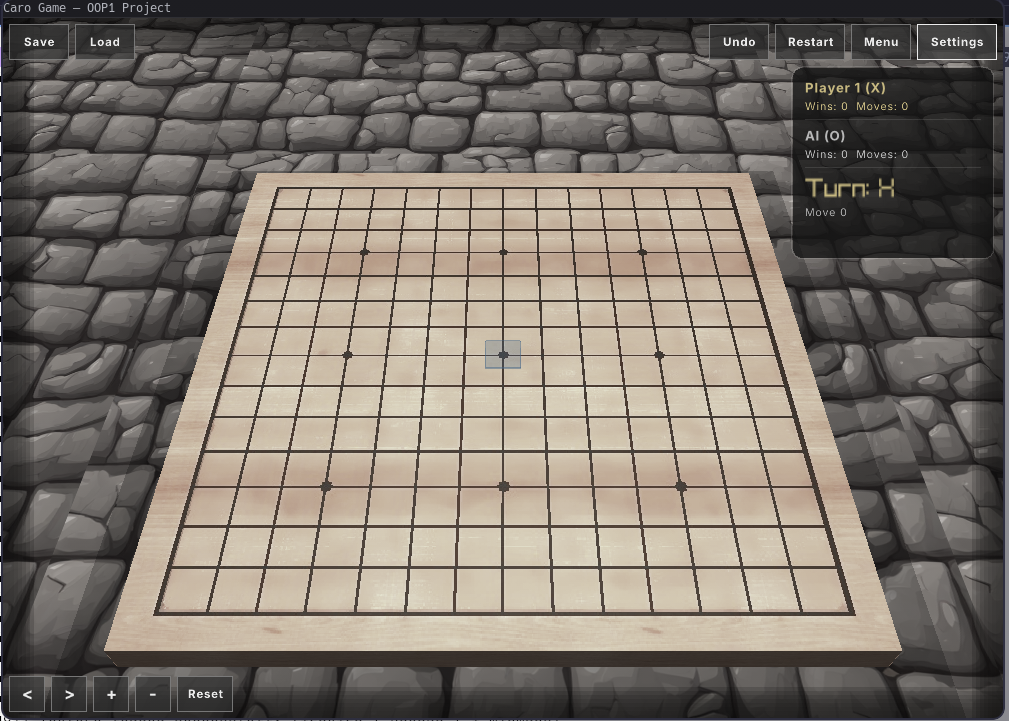
\includegraphics[width=0.72\textwidth]{../../public/init_board.png}
\caption{Bàn cờ khởi đầu — 15×15 ô trống, quân X đi trước (Turn: X). HUD bên phải hiển thị tên hai người chơi, số nước, thời gian đã chơi.}
\end{figure}

\begin{figure}[H]
\centering
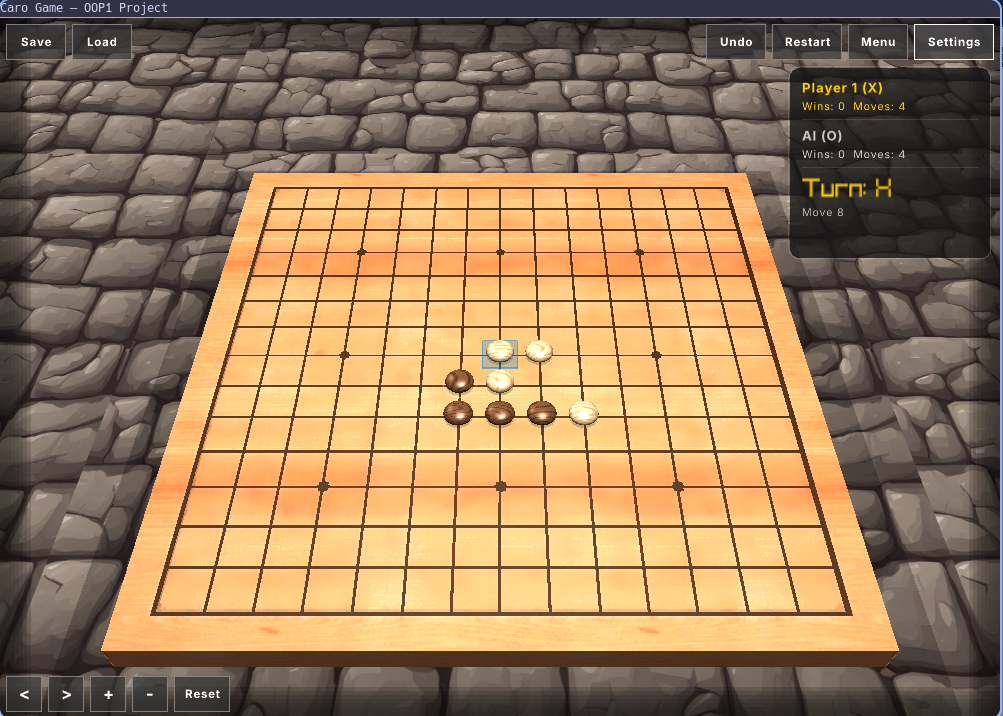
\includegraphics[width=0.72\textwidth]{../../public/some_step.png}
\caption{Giữa ván — các quân X (đen) và O (trắng) đặt thành cụm xoay quanh ô trung tâm. Texture gỗ mỗi ô được nạp độc lập qua worker thread (§4.7) nên bàn không đơn điệu.}
\end{figure}

\begin{figure}[H]
\centering

\includegraphics[width=0.72\textwidth]{../../public/settings.png}
\caption{Settings — chọn chế độ (Player vs AI / Player vs Player) và mức khó AI (Easy / Normal / Hard). Khi ở PvP, dòng "AI Difficulty" bị giảm sáng (xám).}
\end{figure}

\begin{figure}[H]
\centering
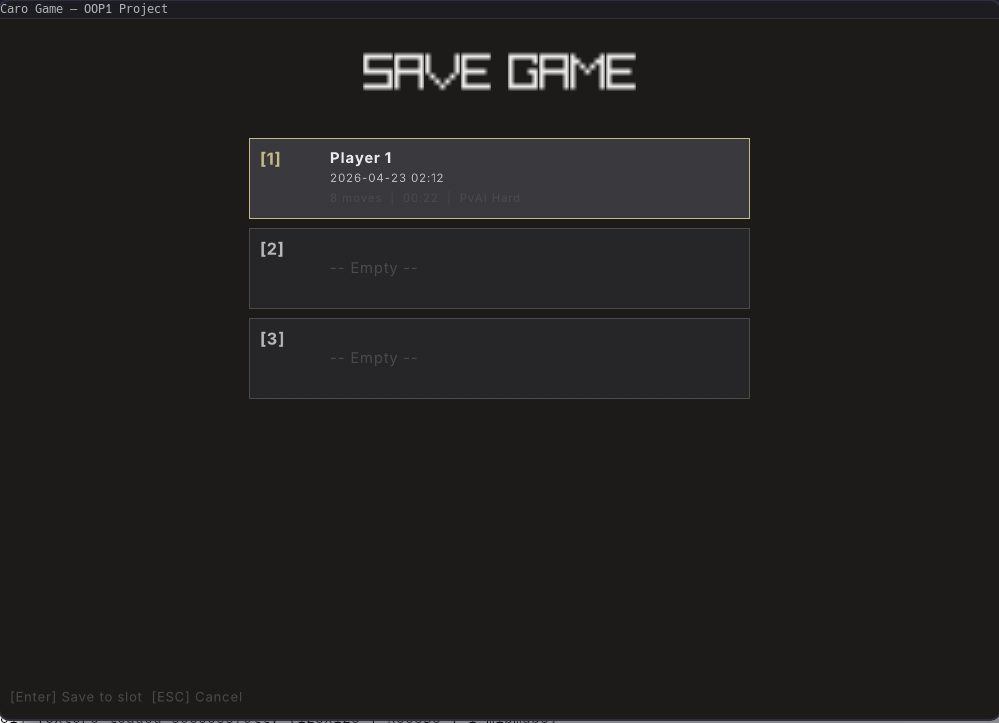
\includegraphics[width=0.72\textwidth]{../../public/save.png}
\caption{Save Game — 3 slot thủ công. Slot 1 đã có dữ liệu (tên Player 1, thời điểm 2026-04-23 02:12, 8 nước đi, chế độ PvAI Hard). Slot đang chọn được highlight viền vàng.}
\end{figure}

\begin{figure}[H]
\centering
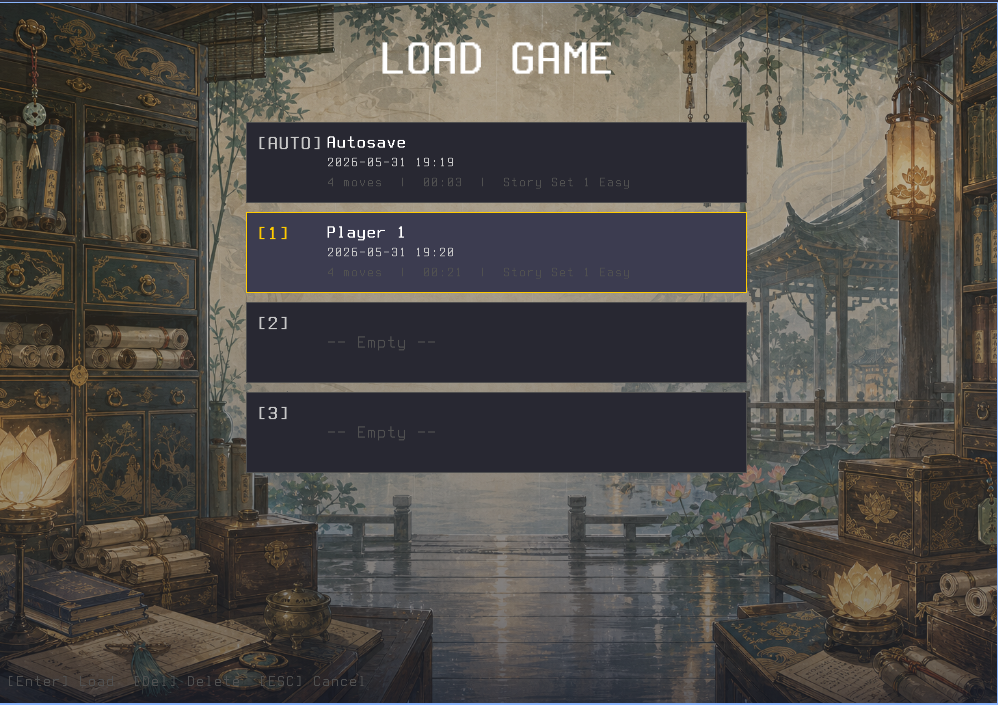
\includegraphics[width=0.72\textwidth]{../../public/load.png}
\caption{Load Game — 4 slot: slot \texttt{AUTO} là autosave ghi đè sau mỗi nước đi, slot [1] là bản lưu thủ công. Mỗi entry hiển thị timestamp, số nước, chế độ chơi.}
\end{figure}

\begin{figure}[H]
\centering
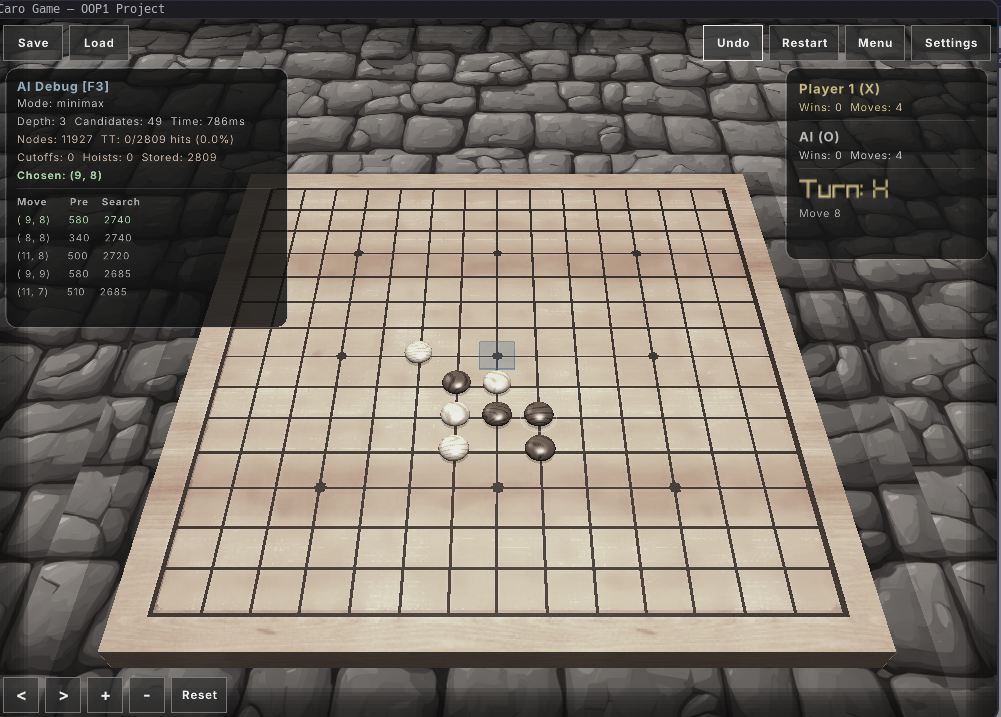
\includegraphics[width=0.72\textwidth]{../../public/debug.png}
\caption{Debug panel (F3) — phía trên trái hiển thị mode Hard, Depth=3, Time=xx ms, Candidates, Nodes, TT probes/hits/cutoffs/hoists, và top-5 nước được AI đánh giá cao nhất kèm điểm tìm kiếm. Dùng để kiểm chứng hoạt động của minimax α-β + TT (§3.5, §3.7).}
\end{figure}

\begin{figure}[H]
\centering
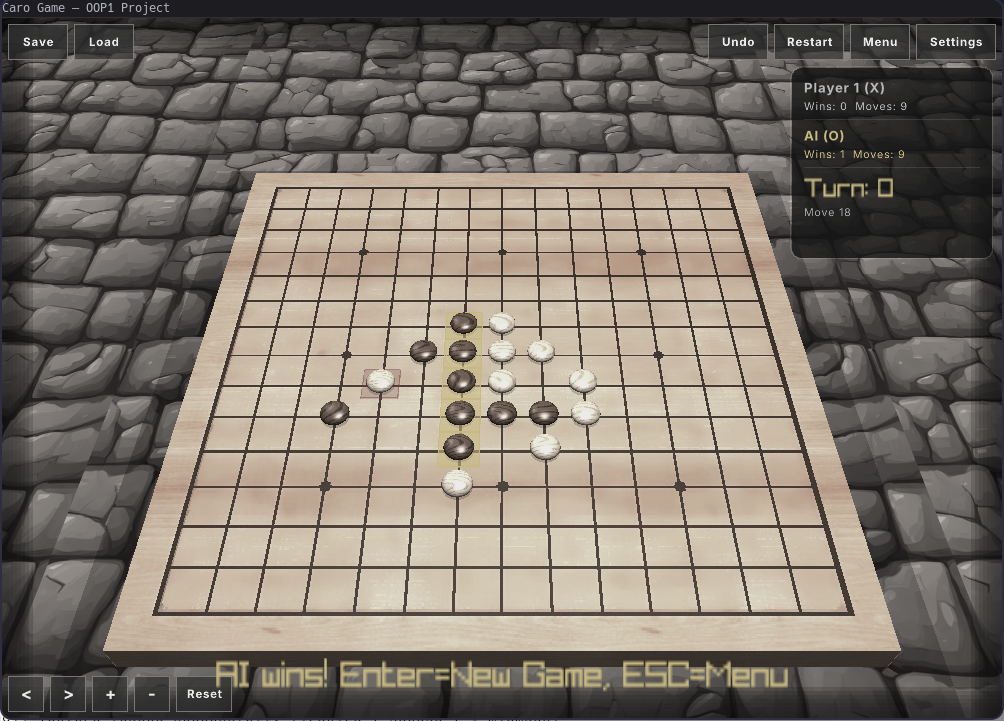
\includegraphics[width=0.72\textwidth]{../../public/ai_win.png}
\caption{Màn hình kết thúc ván — AI đã tạo đường 5 quân thắng theo đường chéo. Banner "AI wins!  Enter=New Game  ESC=Menu" hiện phía dưới.}
\end{figure}
\subsection{6.2 Tổng kết}
\label{sec:orgad88771}

Đồ án hoàn thành \textbf{đầy đủ yêu cầu bắt buộc} (PvP, PvE, check win, save/load, UI) cùng loạt tính năng nâng cao. Ba điểm nổi bật:

\begin{enumerate}
\item \textbf{OOP đúng chuẩn} — \texttt{Player=/=AIPlayer} với virtual \texttt{getMove} là ví dụ trực tiếp của kế thừa + đa hình runtime qua vtable. Phân rã 24 module theo SRP giúp code test được, bảo trì được, mở rộng được.

\item \textbf{Kỹ thuật vượt yêu cầu} — Zobrist hashing, Transposition Table, α-β + move ordering, incremental evaluation, async AI thread, async texture streaming.

\item \textbf{Chất lượng UX} — camera quỹ đạo, Phong shader, hoạt ảnh squash \& stretch, 3 loại particle, win effect, âm thanh — gần chuẩn sản phẩm thương mại.

\item \textbf{Nội dung phong phú, mở rộng không sửa lõi} — chế độ Story 4 chặng có cốt truyện + linh-vật (Chương 5) và Multiplayer LAN/online qua TCP (§2.7) đều cắm vào pipeline \texttt{applyMove} sẵn có, minh chứng sống cho nguyên tắc Open-Closed.
\end{enumerate}

\textbf{Định lượng:} \textasciitilde{}10\,000 LOC, 24 module, 2 file test Catch2, 3 tier AI (+ màn trùm d=4 ở Story) dùng chung pattern table. Build cold \textasciitilde{}180 s, rebuild nóng \textasciitilde{}3 s.
\subsection{6.3 Hạn chế}
\label{sec:org44bfed1}

\begin{enumerate}
\item \textbf{Tier thường giới hạn depth 3} — d=4 có thể mất \textasciitilde{}120 s/nước ở thế cờ xấu nên chỉ dùng cho màn trùm Story (§5.4), không cho chế độ tương tác thường.
\item \textbf{Không có VCF/VCT threat-space search} — đã có khung \texttt{findThreatWin} nhưng chưa integrate vì chưa đủ thời gian test.
\item \textbf{Không có opening book} — AI đầu ván hơi yếu so với các opening chuẩn.
\item \textbf{Multiplayer phụ thuộc relay ngoài} — chế độ online cần một relay server (không kèm trong repo); LAN P2P thì cần hai máy cùng mạng.
\item \textbf{Không có tutorial} — giả định user đã biết luật.
\item \textbf{Settings chỉ 2 trường} — có thể thêm chọn mark, theme skin, volume riêng.
\end{enumerate}
\subsection{6.4 Hướng phát triển}
\label{sec:orgadef64f}

\begin{enumerate}
\item \textbf{VCF/VCT threat search} — hoàn thiện \texttt{findThreatWin} và tích hợp trước fallback minimax.
\item \textbf{Iterative deepening + time limit} — tìm sâu nhất trong 2 s thay vì fix d=3; kèm TT persistence giữa turn.
\item \textbf{Opening book} — \textasciitilde{}500 thế cờ từ self-play hoặc pro games, probe ở 10 nước đầu.
\item \textbf{Hạ tầng mạng hoàn chỉnh} — relay server tự host kèm matchmaking, NAT traversal (STUN/TURN), reconnect và khán giả; nâng cấp từ multiplayer TCP hiện có (§2.7).
\item \textbf{Theme skin} — nhiều bộ texture gỗ, user chọn trong Settings.
\item \textbf{Mobile port} — raylib có backend Android.
\item \textbf{AI Expert tier} — iterative deepening + VCF/VCT + opening book.
\item \textbf{Replay system} — lưu \texttt{moveHistory} đầy đủ, cho xem lại từng nước.
\end{enumerate}
\subsection{6.5 Phân công công việc}
\label{sec:orgfe5091e}

\begin{center}
\begin{tabularx}{\textwidth}{llXl}
Thành viên & MSSV & Phần đảm nhiệm chính & Đóng góp\\
\hline
Nguyễn Hữu Thiện Nhân & 25310023 & Nhóm trưởng. Toàn bộ source code C++ (24 module, \textasciitilde{}10\,000 LOC): kiến trúc, AI, Renderer, UI, Save/Load, âm thanh, Multiplayer, Story Mode, unit test. Soạn nội dung báo cáo kỹ thuật. & \_\_\_\_\_\%\\
Bùi Thị Minh Hằng & 25310057 & Thiết kế slide thuyết trình; biên tập, dàn trang và kiểm tra chính tả báo cáo; ghi video demo. & \_\_\_\_\_\%\\
Phạm Ngọc Trâm & 25310043 & Thiết kế slide thuyết trình; chụp / tổng hợp ảnh minh họa; hỗ trợ dàn trang báo cáo. & \_\_\_\_\_\%\\
\textbf{Tổng} &  &  & \textbf{100 \%}\\
\end{tabularx}
\end{center}

\emph{(Tỉ lệ \% điền sau buổi sync cuối trước khi nộp.)}

\noindent\rule{\textwidth}{0.5pt}
\section{Tài liệu tham khảo}
\label{sec:orgf2bfa83}

{[}1] \textbf{Raysan5} (2024). \emph{raylib 5.5 Documentation}. \url{https://www.raylib.com}

{[}2] \textbf{Russell, S. \& Norvig, P.} (2020). \emph{Artificial Intelligence: A Modern Approach}, 4th ed. Pearson. — Ch.5 Adversarial Search: Minimax, α-β, TT, Move Ordering.

{[}3] \textbf{Allis, L. V.} (1993). \emph{Searching for Solutions in Games and Artificial Intelligence}. Ph.D. dissertation, University of Limburg. — §4: Gomoku/Renju, threat-space search, VCF/VCT.

{[}4] \textbf{Zobrist, A. L.} (1970). \emph{A New Hashing Method with Application for Game Playing}. Tech. Rep. 88, Univ. of Wisconsin.

{[}5] \textbf{Wikipedia} (2025). \emph{Horizon effect}. \url{https://en.wikipedia.org/wiki/Horizon\_effect}

{[}6] \textbf{ISO/IEC 14882:2014} — C++14 Standard. \url{https://en.cppreference.com}

{[}7] \textbf{Kitware} (2024). \emph{CMake 3.16+ Documentation}. \url{https://cmake.org/documentation}

{[}8] \textbf{Preshing, J.} (2014). \emph{The World's Simplest Lock-Free Hash Table}. \url{https://preshing.com/20130605/}

{[}9] \textbf{catchorg} (2024). \emph{Catch2 v3}. \url{https://github.com/catchorg/Catch2}

{[}10] \textbf{IEEE 802.3} — CRC-32 polynomial \texttt{0xEDB88320}.

\noindent\rule{\textwidth}{0.5pt}

\emph{— Hết báo cáo —}
\end{document}
